\section{Wychwytywanie $CO_2$}

\begin{frame}{Jak działa technologia CCS?}
    \begin{figure}
        \centering
        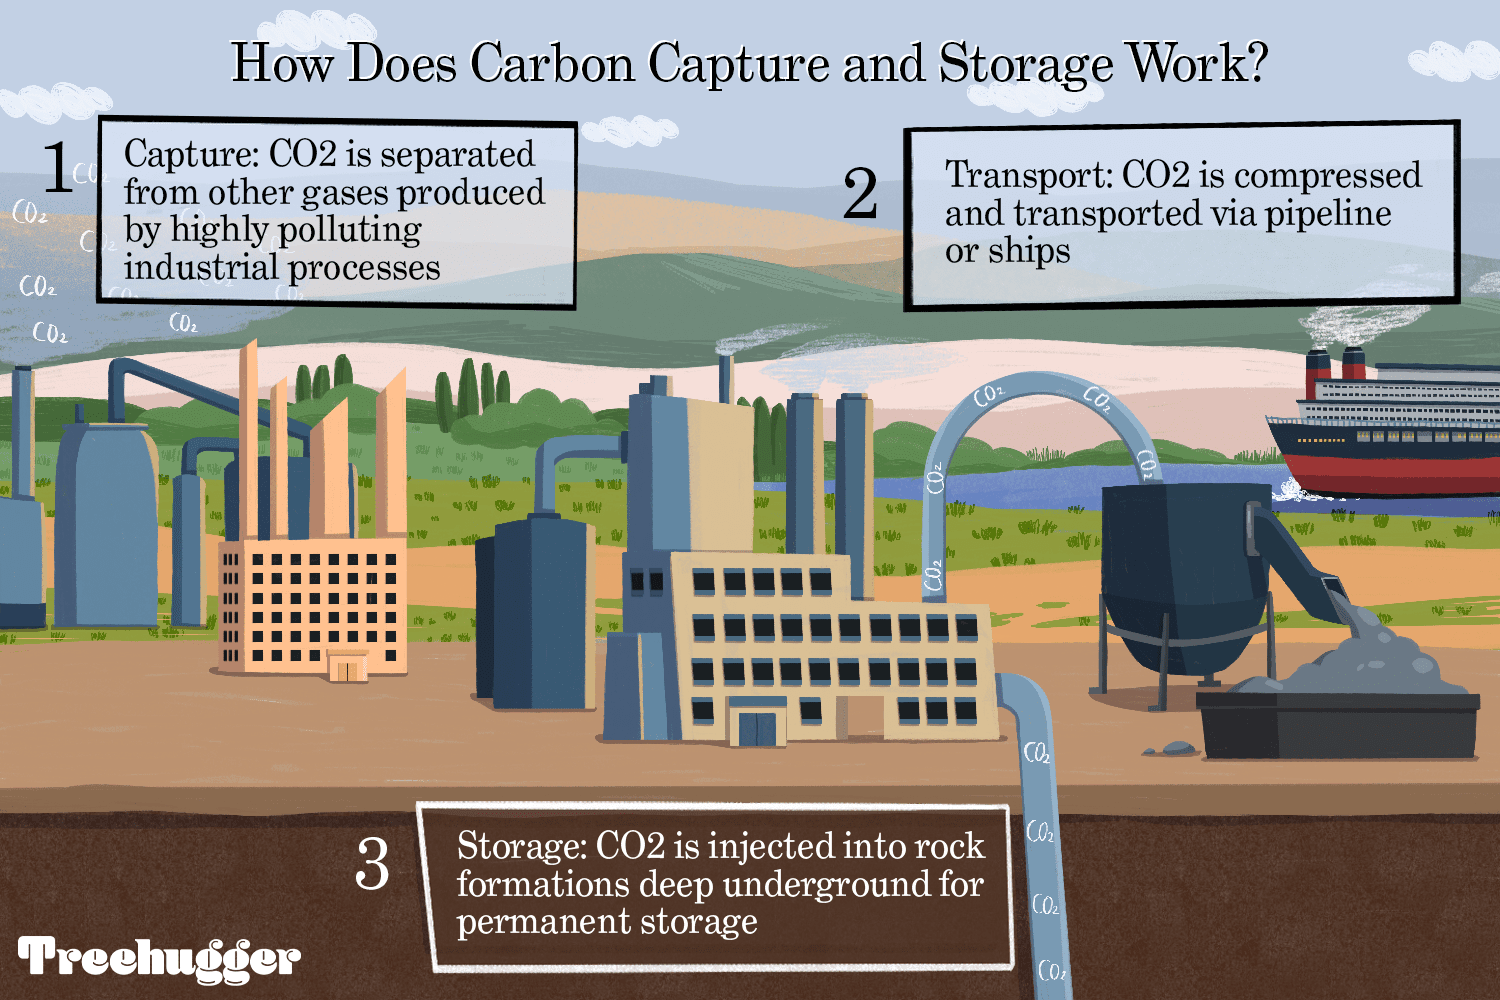
\includegraphics[width=0.6\textwidth, frame]{images/CCS_treehugger.png}
    \end{figure}
\end{frame}

\begin{frame}{CCS: Wychwytywanie (Capture)}
    \begin{figure}
        \centering
        % 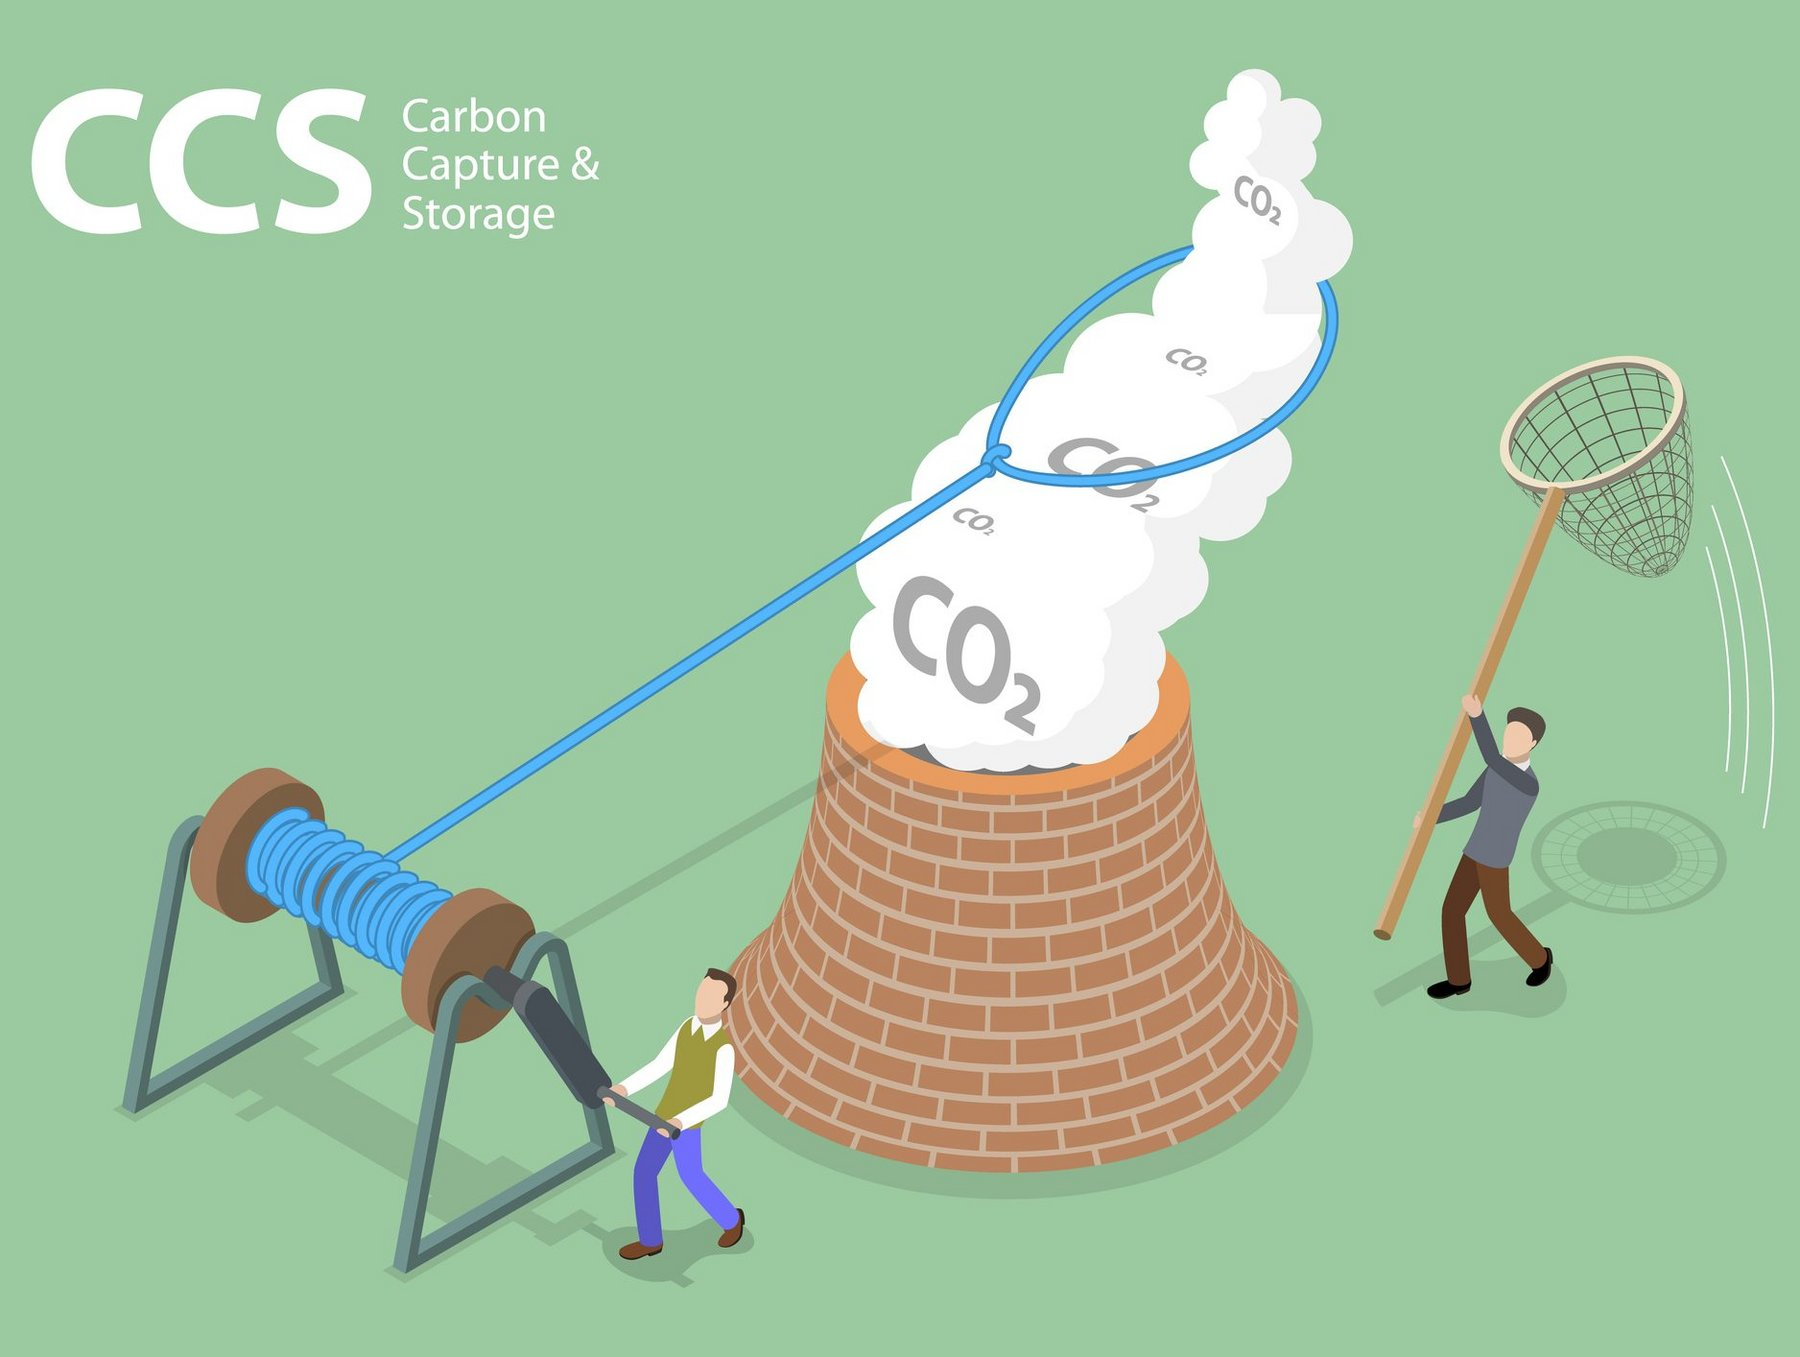
\includegraphics[width=0.6\textwidth, frame]{images/CCS_illustration_gettyimages.jpg}
        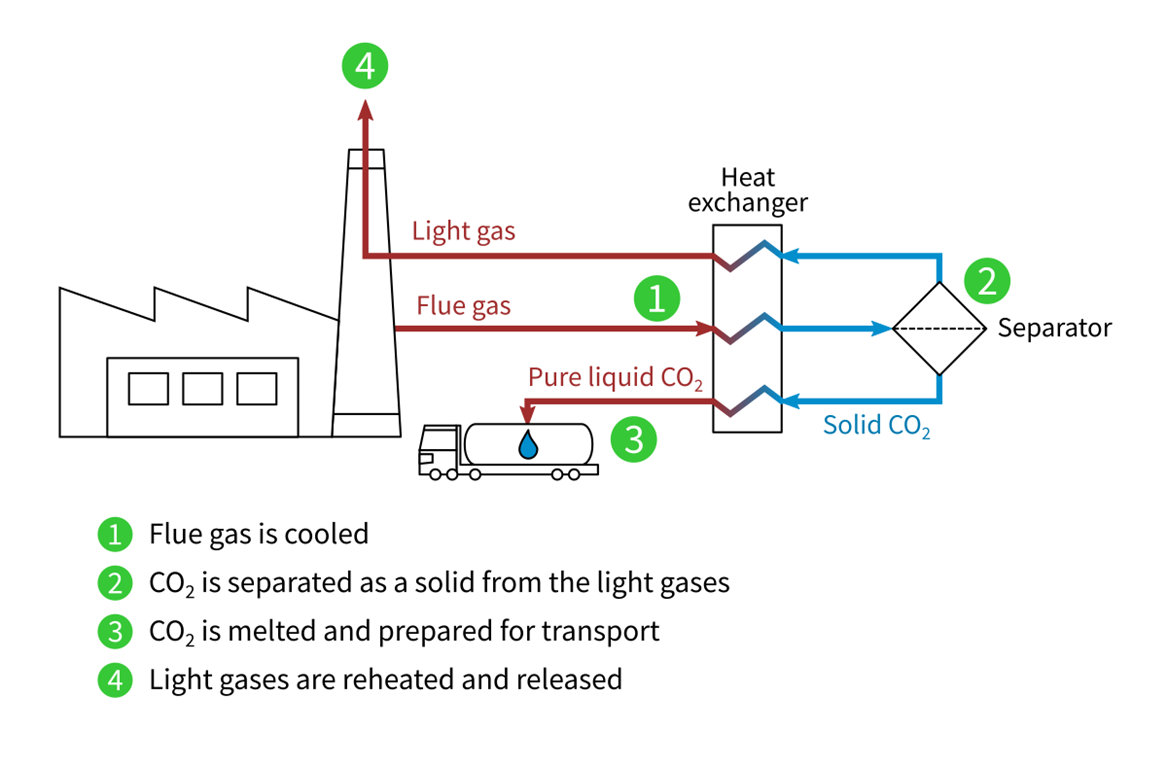
\includegraphics[width=0.7\textwidth, frame]{images/carbon-capture-how-it-works.png}

        % 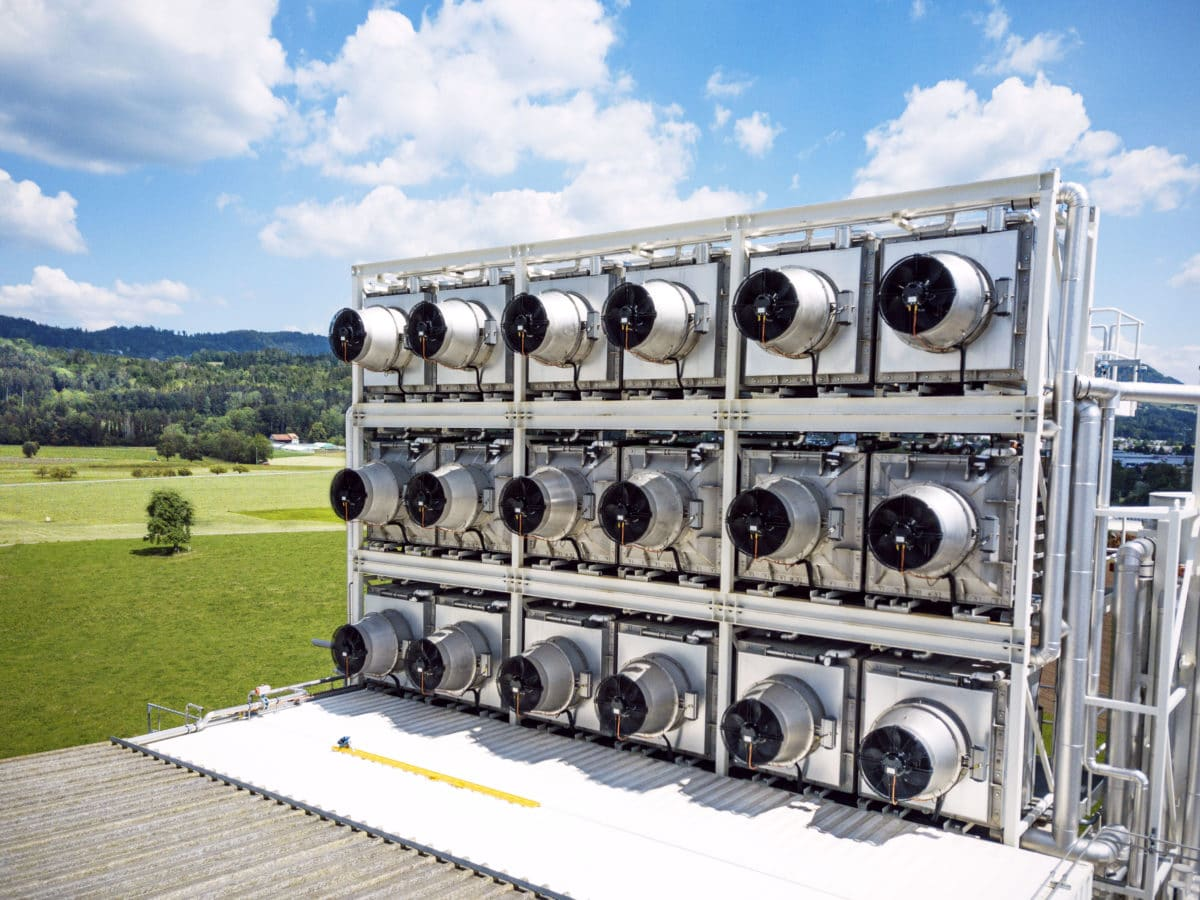
\includegraphics[width=0.6\textwidth, frame]{images/carbon_capture_from_air.jpeg}
    \end{figure}
\end{frame}

\begin{columnframe}{CCS: Transport}
    \begin{column}{0.5\textwidth}
        \begin{figure}
            \centering
            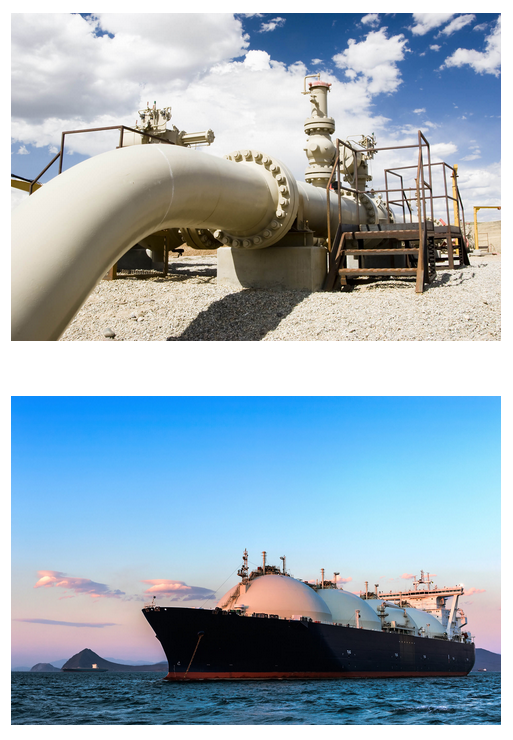
\includegraphics[width=0.6\textwidth, frame]{images/co2_transport.png}
        \end{figure}
    \end{column}
    \begin{column}{0.5\textwidth}
        \begin{itemize}
            \item Transport CO$_2$
                  odbywa się w podobny sposób jak transport gazu ziemnego lub ropy naftowej - rurociągami, cysternami, statkami.
        \end{itemize}
    \end{column}
\end{columnframe}

\begin{columnframe}{CCS: Magazynowanie (Storage)}
    \begin{column}{0.5\textwidth}
        \begin{itemize}
            \item Wychwytane CO$_2$ jest przechowywane w geologicznych formacjach, takich jak pustynie solne.
            \item Alternatywnie może być wykorzystane w szeroko pojętym przemyśle chemicznym.
        \end{itemize}
    \end{column}
    \begin{column}{0.5\textwidth}
        \begin{figure}
            \centering
            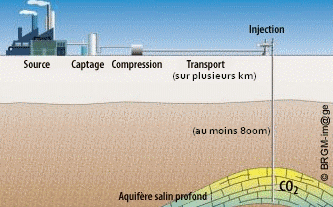
\includegraphics[width=0.9\textwidth, frame]{images/La-chaine-de-valeur-transporter-le-CO2.jpg}
        \end{figure}
    \end{column}
\end{columnframe}


\begin{columnframe}{Zalety CCS}
    \begin{column}{0.5\textwidth}
        \begin{figure}
            \centering
            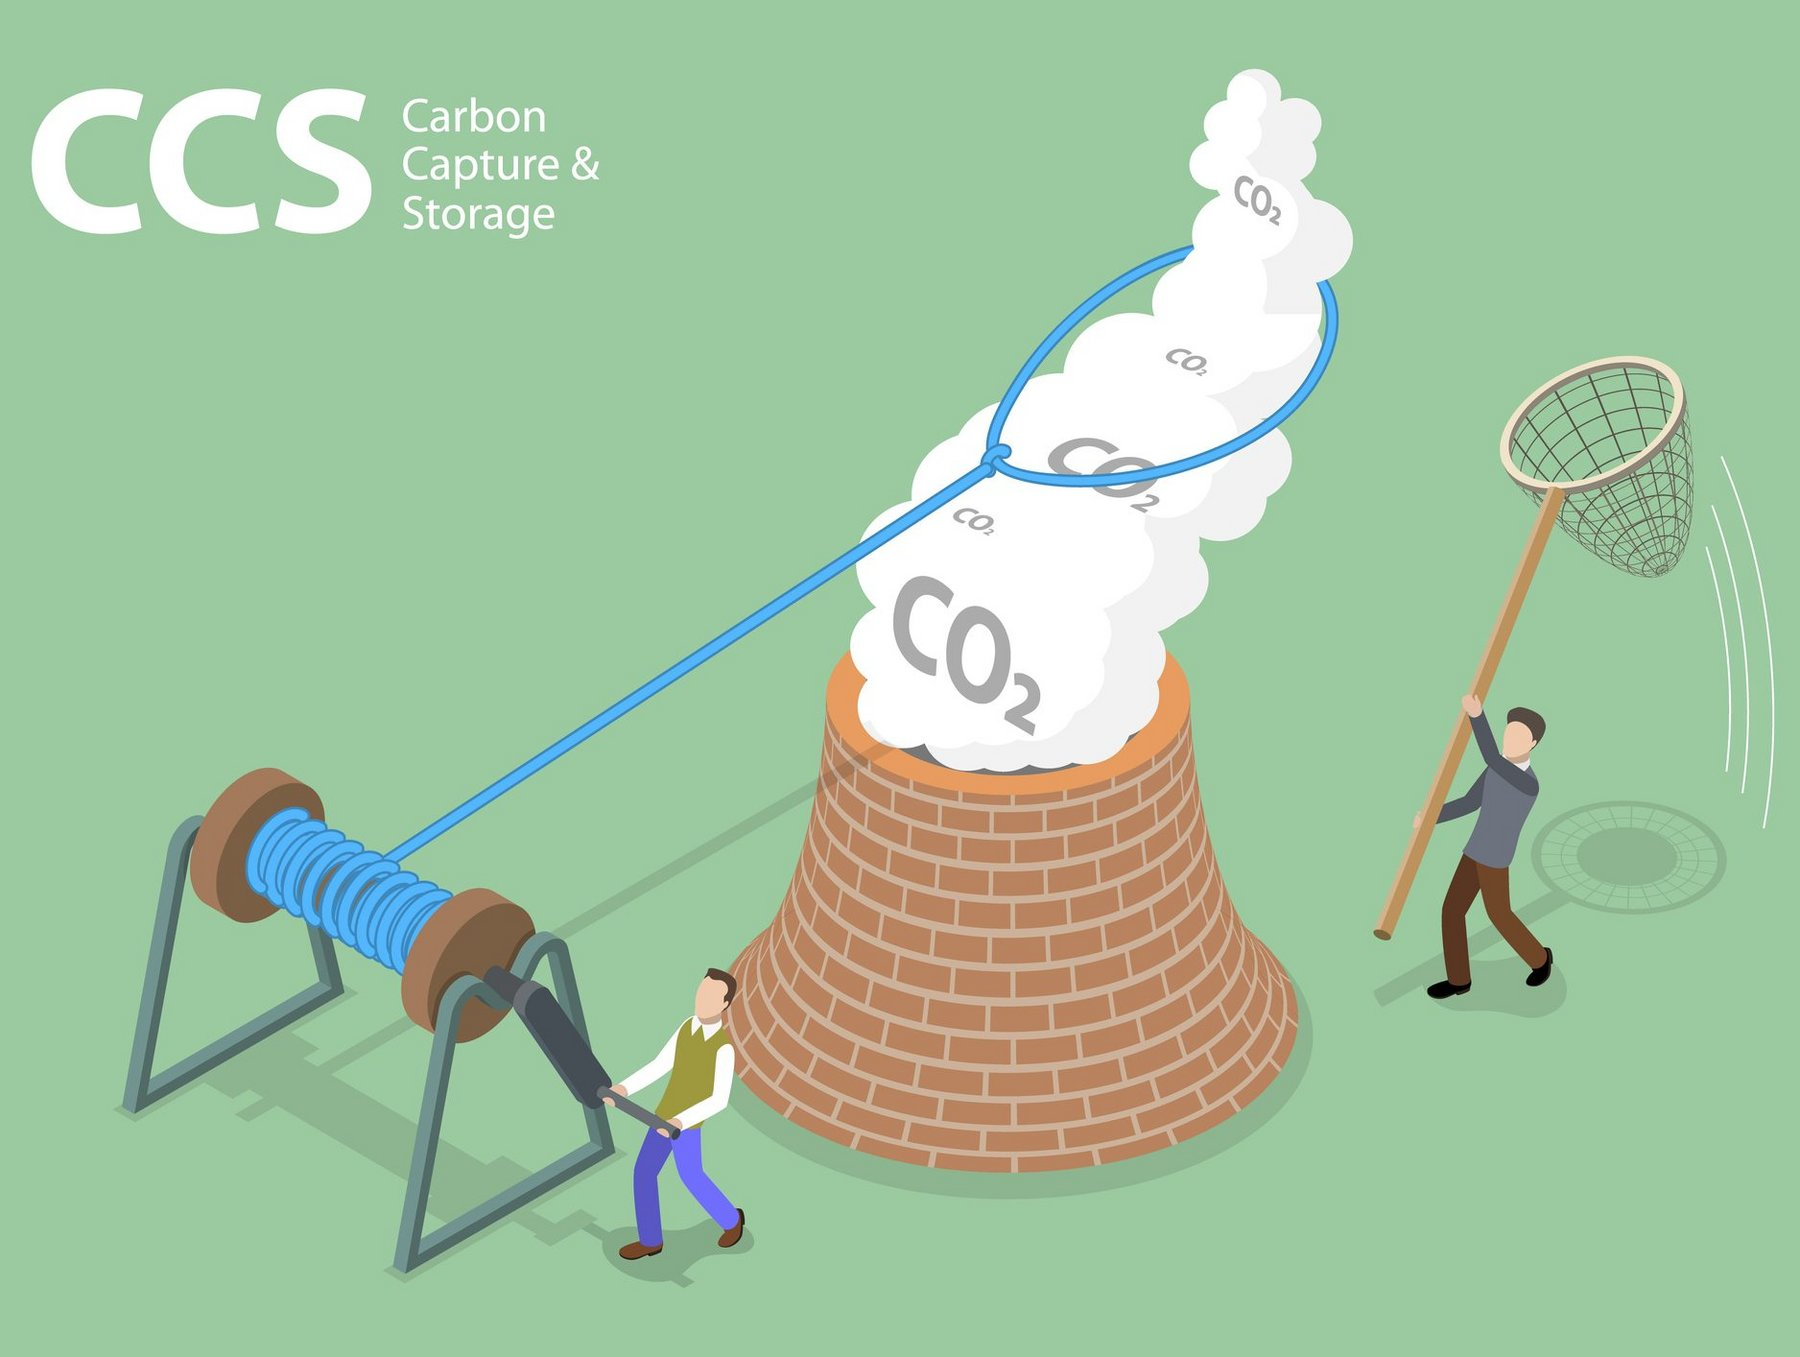
\includegraphics[width=0.8\textwidth, frame]{images/CCS_illustration_gettyimages.jpg}
        \end{figure}
    \end{column}
    \begin{column}{0.5\textwidth}
        \begin{itemize}
            \item Zalety CCS: redukcja emisji w sektorach trudnych do dekarbonizacji
            \item Aktywna redukcja CO$_2$ w atmosferze
        \end{itemize}
    \end{column}
\end{columnframe}

\begin{columnframe}{Problemy CCS}
    \begin{column}{0.5\textwidth}
        \begin{itemize}
            \item Koszty
            \item Duże zużycie energii
            \item Ryzyko wycieków
            \item Wyzwania techniczne
            \item Brak regulacji
            \item Brak motywacji ekonomicznej - CO$_2$ nie generuje zysków pieniężnych
        \end{itemize}
    \end{column}
    \begin{column}{0.5\textwidth}
        \begin{figure}
            \centering
            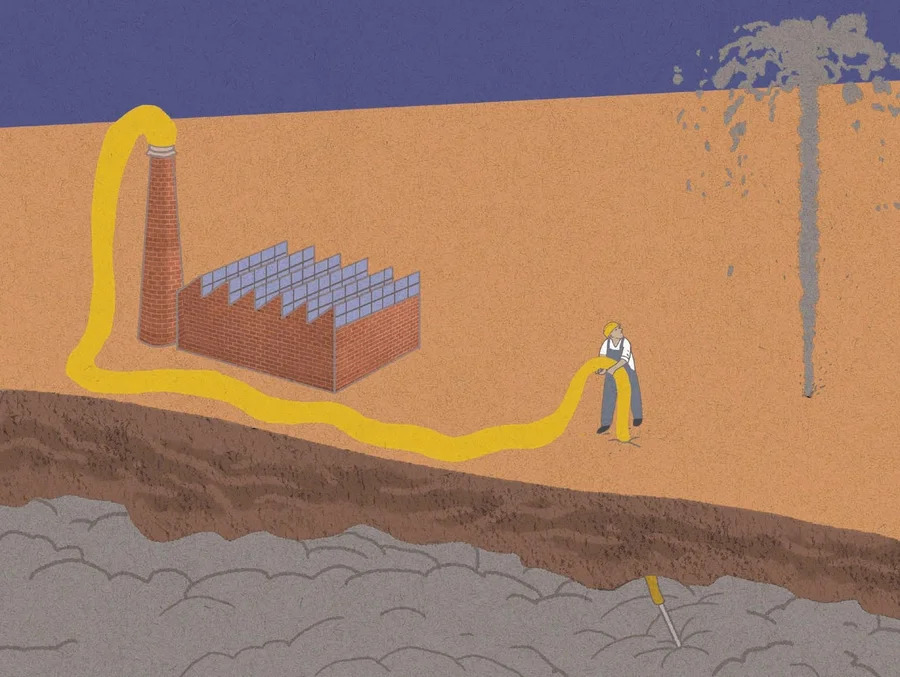
\includegraphics[width=0.8\textwidth, frame]{images/anti_ccs_propaganda.jpg}
        \end{figure}
    \end{column}
\end{columnframe}